\section{Классификация изображений датасета MNIST}

Теперь решим задачу классификации датасета MNIST. Опишем общий алгоритм \ref{classification-pipeline}, который лежит в основе решения задачи.

\medskip
\begin{algorithm}[H]
	\small
	\SetAlgoLined
	\KwData{Набор изображений рукописных цифр}
	\KwResult{Алгоритм, определяющий рукописную цифру}
	\ForEach{изображения из выборки}{
		Построить фильтрации;
		
		Найти персистентные гомологии, построить диаграмму персистентости;
		
		Получить топологические признаки из диаграммы персистентности;
	}
	
	На наборе полученных признаков обучить модель машинного обучения;
	\caption{Общий алгоритм решения задачи классификации}
	\label{classification-pipeline}
\end{algorithm}
\medskip

Как видно из алгоритма, основным этапом является получение топологических признаков. На их основе и будет обучаться модель машинного обучения. Признаки получаются из диаграммы устойчивости различными методами, поэтому для одного изображения можно получить сразу несколько признаков по одной диаграмме. С другой стороны, персистентные гомологии, а значит и диаграмму устойчивости, можно считать для различных фильтраций одного и того же изображения. Таким образом на основе одного изображения можно сразу получить большое количество признаков, строя по ней различные фильтрации и различными способами векторизуя диаграмму. В данной работе использовался подход, изображенный на рис. \ref{pipeline}

\begin{figure}[!htbp]
	\begin{center}
		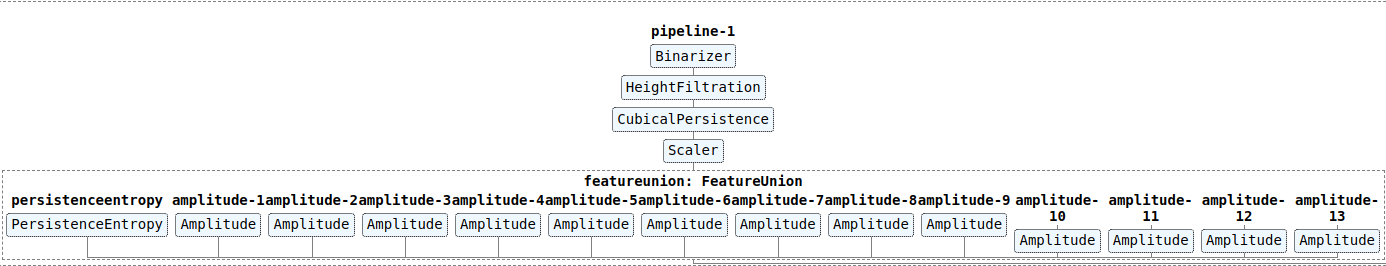
\includegraphics[width=\textwidth]{pipelineDiagram.png}\\
		\caption{Алгоритм получения признаков для Height Filtration}
		\label{pipeline}
	\end{center}
\end{figure}

Опишем подробнее алгоритм получения признаков. Первым шагом является бинаризация изображения с заранее выбранным пороговым значением(в данной работе значение порога равнялось $0.4$). Это нужно для того, чтобы далее воспользоваться специальными методами фильтрации, которые работают именно с бинарным изображением. Бинарным изображением будет называть отображение $B: \mathbb{R}^d \to \{0, 1\}$.

Далее по бинарному изображению $B$ строятся специальные фильтрации. По большому счету фильтрации можно воспринимать как трансформации бинарного изображения обратно в черно-белое, пропущенное через специальный фильтр. Так как в результате получается черно-белое изображение, то можно считать устойчивые гомологии сразу для самой картинки, но обычно построение черно-белого изображения через бинаризацию и фильтрацию наиболее сильно подчеркивает различные топологические особенности. В данном алгоритме использовалась т.н. фильтрация по высоте, а также радиальная фильтрация(рис. \ref{filtration-comparison}). 

\begin{figure}[!htbp]
	\begin{center}
		\includegraphics[width=0.5\textwidth]{example-image-a}\\
		\caption{Черно-белые изображения, полученные с помощью различных фильтраций. Для наглядности, была использована цветная гамма для представления черно-белых значений}
		\label{filtration-comparison}
	\end{center}
\end{figure}
Фильтрация по высоте(Height filtration) -- это отображение $H: I \to \mathbb{R}$, где $I$ -- это бинарное изображение в общем случае размерности $d$(в нашем случае размерность равна $2$), которое каждому пикселю изображения $p$ сопоставляет расстояние до гиперплоскости, которая определена вектором $v$ длины $1$, заданным заранее:
\[
H: p \mapsto 
	\left\{
		\begin{array}{ll}
			\langle p,v \rangle, & \text{если } B(p) = 1, \\
			H_\infty, & \text{иначе,}
		\end{array}
	\right.
\]
где $H_\infty$ -- это значение фильтрации $H$ самого дальнего пикселя изображения до гиперплоскости.


Радиальная фильтрация(Radial filtration) -- это отображение $R: I \to \mathbb{R}$, которое каждому пикселю изображения сопоставляет расстояние до выбранного заранее центра $c$:
\[
	R: p \mapsto 
		\left\{
			\begin{array}{ll}
				\norm{c - p}_2, & \text{если } B(p) = 1, \\
				R_\infty, & \text{иначе,}
			\end{array}
		\right.
\]
где $R_\infty$ -- это расстояние самого дальнего пикселя до центра. То есть фильтрация строится исходя из значения некоторой радиальной функции от пикселя $p$, у которого $B(p)=1$.

Так как вектор направления для фильтрации по высоте и центр для радиальной фильтрации задается заранее, то можно формировать различные фильтрации при различных значениях вектора направления и центра. В данном алгоритме фильтрация по высоте строилась с $8$ различными значениями для вектора направления, а радиальная фильтрация строилась с $9$ различными значениями для центра. Таким образом, для одного изображения получалось 17 фильтраций.

\begin{figure}[!htbp]
	\begin{center}
		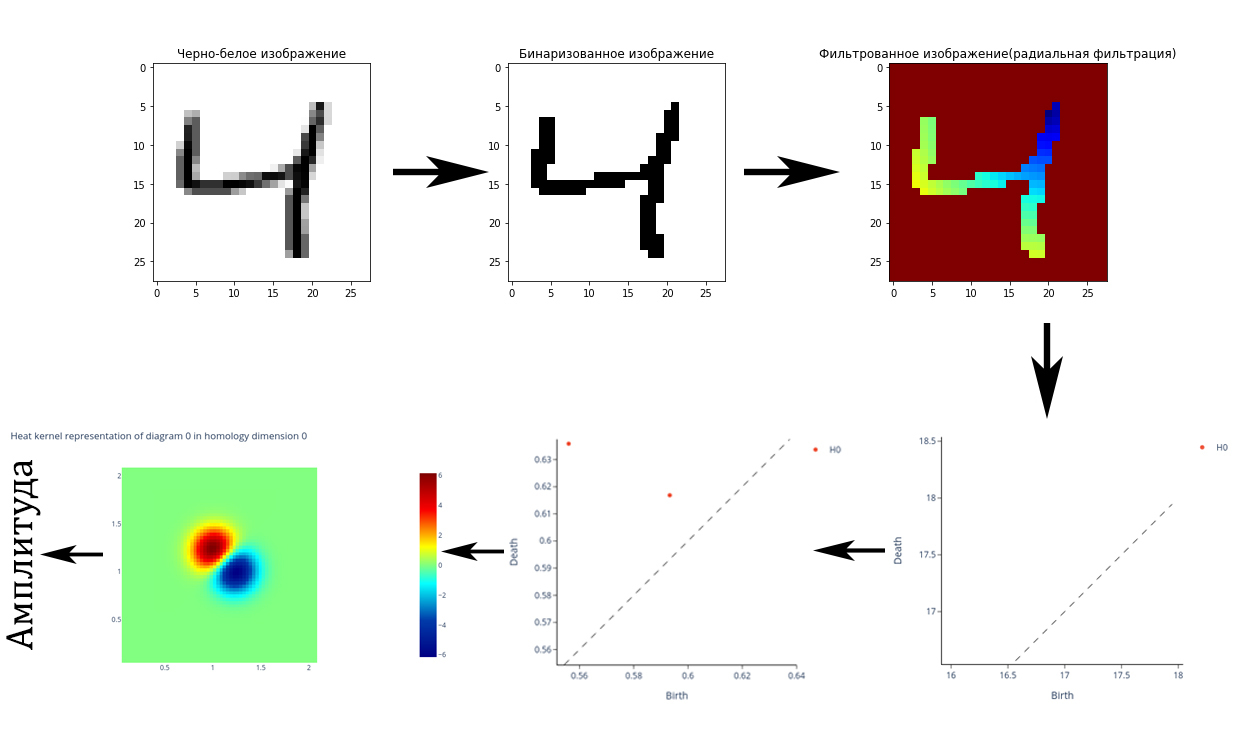
\includegraphics[width=0.75\textwidth]{pipe.jpg}\\
		\caption{Пример работы алгоритма}
		\label{example}
	\end{center}
\end{figure}

Далее для каждой из полученных фильтраций вычислялись устойчивые гомологии $0$ и $1$ размерности, а по ним строились диаграммы персистентности, которые далее были приведены к одному и тому же масштабу. В свою же очередь, для каждой диаграммы вычислялись 14 признаков: персистентная энтропия и 13 амплитуд для различных векторных представлений. Таким образом, для одной картинки получалось $17 \times 2 \times 14 = 476$ признаков. На рис. \ref{example} представлен пример работы алгоритма для одного бинарного изображения из датасета.
